\chapter{Resultados}
	
	\section{Análisis de datos de las variables climáticas propuestas}
	
	Los datos utilizados fueron obtenidos de \textit{NASA Langley Research Center (LaRC) POWER Project} financiado por el Programa de Ciencias de la Tierra/Ciencias Aplicadas de la NASA.
	
		\subsection{Radiación solar de onda corta}
			
			En la~\cref{fig:SFC_SW_DWN} observamos que de marzo a septiembre tenemos los niveles más altos de \acrlong{roc}.
	
			\begin{figure}[H]
				\centering
				\begin{subfigure}[t]{0.45\linewidth}
					\centering
					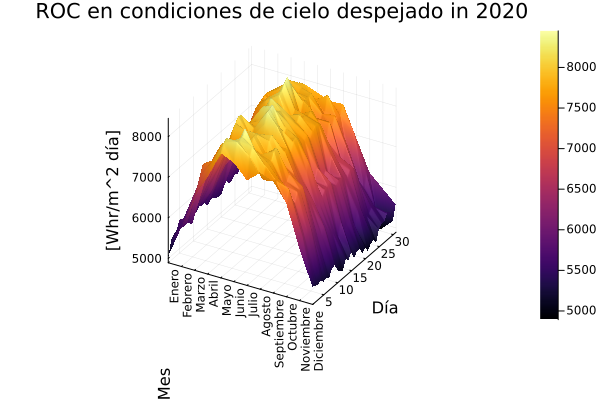
\includegraphics[
						width=\linewidth,
						height = 60mm,
						keepaspectratio
					]{Resultados/DataAnalysis/CLRSKY_SFC_SW_DWN_surface_2020_3d.png}
					\caption{Irradiación de onda corta total recibida por día en condiciones de cielo despejado durante el 2020 sobre el lugar seleccionado}
					\label{fig:CLRSKY_SFC_SW_DWN_surface_2020_3d}
				\end{subfigure}
				\hfill
				\begin{subfigure}[t]{0.45\linewidth}
					\centering
					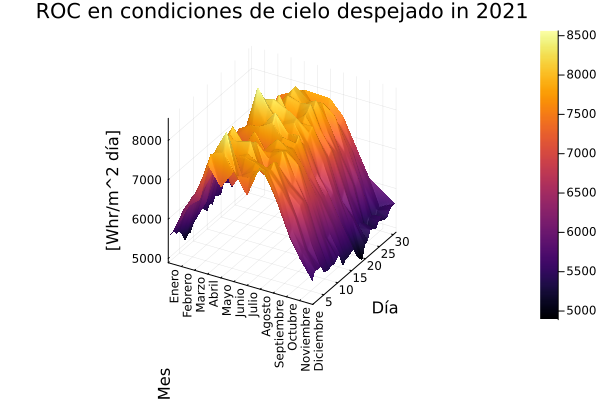
\includegraphics[
						width=\linewidth,
						height = 60mm,
						keepaspectratio
					]{Resultados/DataAnalysis/CLRSKY_SFC_SW_DWN_surface_2021_3d.png}
					\caption{Irradiación de onda corta total recibida por día en condiciones de cielo despejado durante el 2021 sobre el lugar seleccionado}
					\label{fig:CLRSKY_SFC_SW_DWN_surface_2021_3d}
				\end{subfigure}
			\end{figure}
			
			\begin{figure}[H]\ContinuedFloat
				\begin{subfigure}[t]{0.45\linewidth}
					\centering
					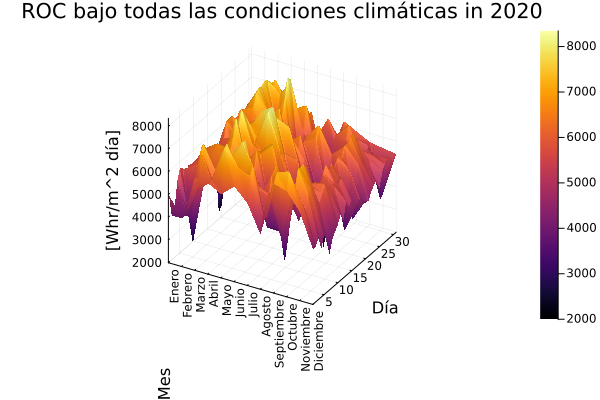
\includegraphics[
						width=\linewidth,
						height = 60mm,
						keepaspectratio
					]{Resultados/DataAnalysis/ALLSKY_SFC_SW_DWN_surface_2020_3d.png}
					\caption{Irradiación de onda corta total recibida por día bajo todas las condiciones climáticas durante el 2020 sobre el lugar seleccionado}
					\label{fig:ALLSKY_SFC_SW_DWN_surface_2020_3d}
				\end{subfigure}
				\hfill
				\begin{subfigure}[t]{0.45\linewidth}
					\centering
					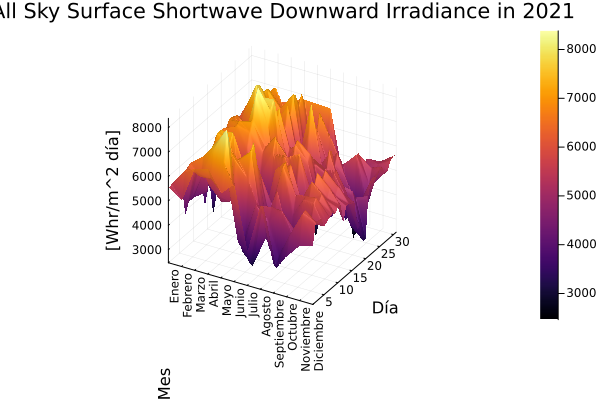
\includegraphics[
						width=\linewidth,
						height = 60mm,
						keepaspectratio
					]{Resultados/DataAnalysis/ALLSKY_SFC_SW_DWN_surface_2021_3d.png}
					\caption{Irradiación de onda corta total recibida por día bajo todas las condiciones climáticas durante el 2021 sobre el lugar seleccionado}
					\label{fig:ALLSKY_SFC_SW_DWN_surface_2021_3d}
				\end{subfigure}
				\caption{Irradiación de onda corta recibida en el lugar físico de experimentación durante 2020 y 2021}
				\label{fig:SFC_SW_DWN}
			\end{figure}
			
%%%%%%%%%%%%%%%%%%%%%%%%%%%%%%%%%%%%%%%%%%%%			
	
	